\section{Aufbau}\label{sec:aufbau}
Der verwendete Germaniumdetektor hat die Form eines Zylinders mit einem Durchmesser von $d = \SI{45}{\milli\meter}$ und einer Länge von $l = \SI{39}{\milli\meter}$ wie in \autoref{fig:detector} zu sehen. Die äußere Oberfläche des Detektors ist durch Eindiffusion von Lithium-Ionen stark n-dotiert, wodurch sie leitfähig wird. Diese n-dotierte Schicht hat eine Dicke von $\SI{5}{\milli\meter}$

Als Sensor dient ein extrem reiner Germaniumkristall mit einer sehr niedrigen Akzeptorendichte von $ n_A \approx 10^{10} \mathrm{Atome/cm^3}$. Zusätzlich ist der Detektor so aufgebaut, dass eine koaxiale Bohrung in der Mitte des Detektorkristalls vorhanden ist. Die innere Oberfläche dieser Bohrung ist mit einer $\SI{20}{\micro\meter}$ starken Goldschicht beschichtet, die einen Metall-Halbleiter-Kontakt bildet.

Der gesamte Detektorkristall wird von einer Schutzhaube aus Aluminium umgeben. Diese Schutzhaube stellt sicher, dass die einfallenden Photonen sowohl die Aluminiumhülle als auch die Lithium-dotierte Oberfläche durchdringen müssen, bevor sie im Germaniumkristall nachgewiesen werden können. Dies führt zu einer niedrigen Nachweisgrenze für Gammaenergien im Bereich von etwa $\SI{40}{\kilo\eV}$, wie bereits erwähnt.

\begin{figure}[h!]
    \centering
    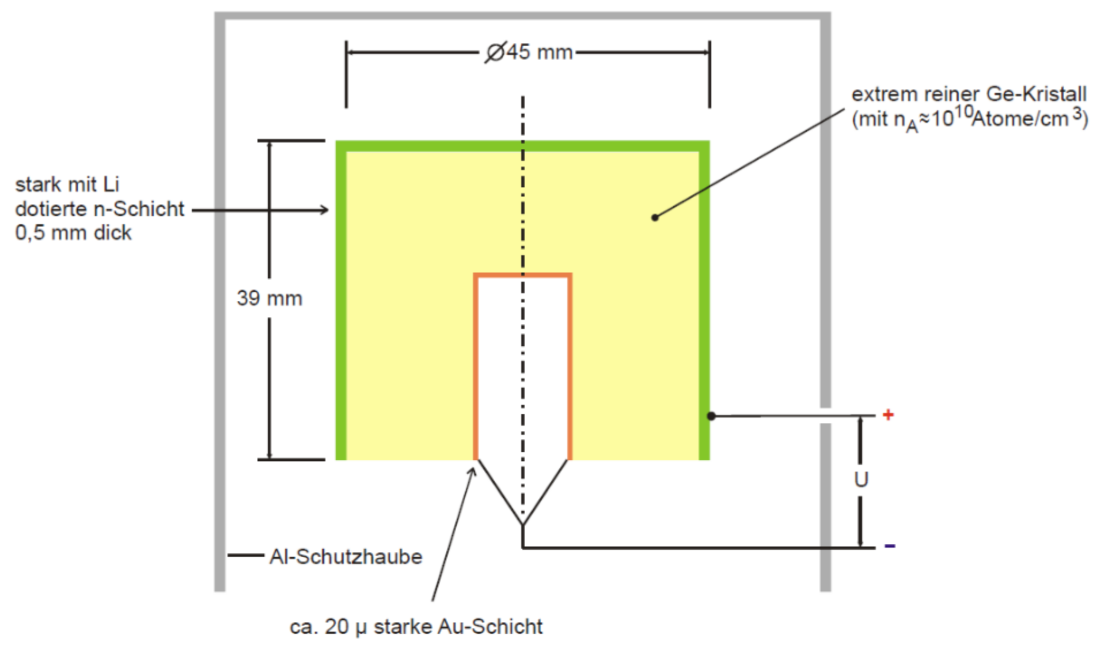
\includegraphics[width=0.8\textwidth]{Ressourcen/detector.png} % Platzhalter für die Abbildung
    \caption{Querschnitt eines koaxialen Germaniumdetektors.\cite{anleitung}}
    \label{fig:detector}
\end{figure}